\documentclass[12pt]{article}

\usepackage{pdflscape}
\usepackage[margin=0.8in]{geometry}
\usepackage{titling}
\usepackage{graphicx} %Required for diagrams
\usepackage[hidelinks]{hyperref}
\usepackage{color}
\usepackage{framed}

\begin{document}

\begin{titlepage}
	\begin{center}
		
		\begin{figure}[t]
			\centering
			
\includegraphics[width=350px]{images/UP_Logo.png}
		\end{figure}
		
		% Title
		\textsc{\large Project Tender} \\ 
		\vspace{2cm}
		\textbf{\Huge Project: RMB's Data Lake} \\ 
		\textsc{\large Client: RMB} \\ 
		\vspace{2cm}
		\textbf{\Huge Team: Team Name } \\ 
		
		%\begin{minipage}{0.4\textwidth}s
		\begin{flushright} \large
			Armand Pieterse \emph{u12167844} \newline
			Kgomotso Sito 		\emph{u12243273} \newline
			student name		\emph{uXXXXXXXX} \newline
			Sphelele Malo 	\emph{u12247040} \newline
			\end{flushright}
		%\end{minipage}
		\textsc{\small Department of Computer Science, University of Pretoria}
		
		\vfill
		
	Here's a link to \href{https://github.com/SpheMalo/COS-301-Main-Project.git}{GitHub}.\\
	\url{https://github.com/SpheMalo/COS-301-Main-Project.git}

	\vfill

	{\large \today}		
		
		
	\end{center}
\end{titlepage}


\newpage
\tableofcontents

\newpage

\section{The Team}

\begin{figure}[h]
			\centering
			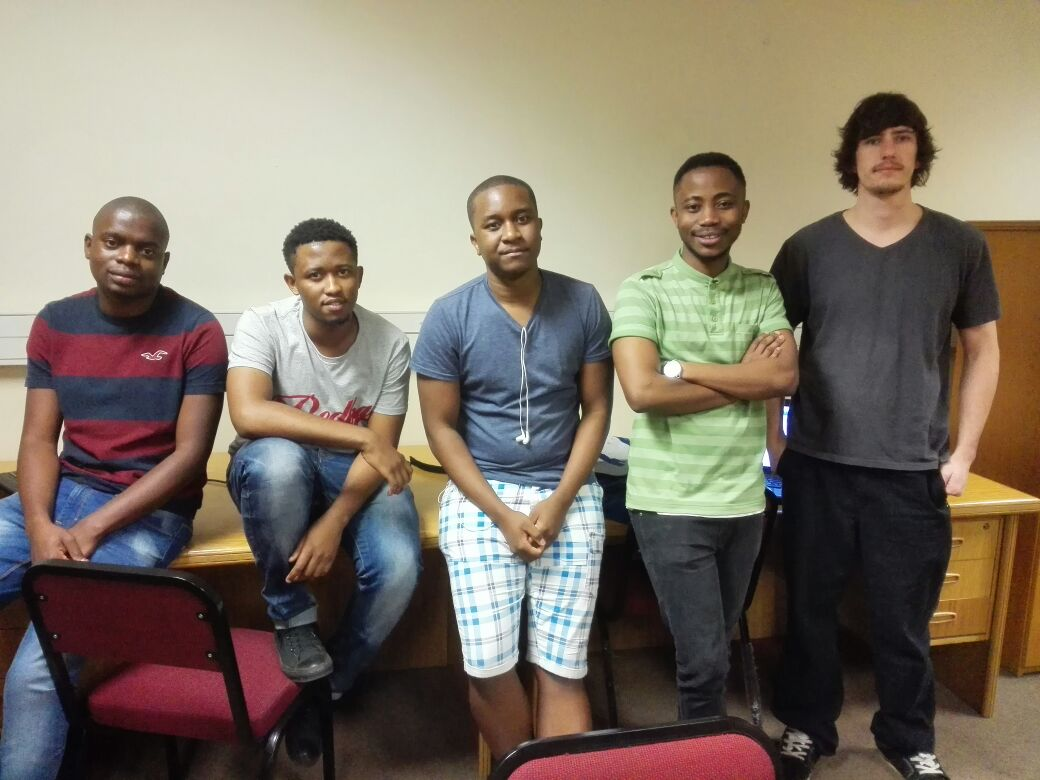
\includegraphics[width=450px]{images/group.jpg}
\end{figure}
		
		\begin{center}
		\textbf{\Huge Introducing Creativate }
		
		\textbf{\emph{Where Creativity meets Innovation}}
		\end{center}
		\newpage

%Jimmy%
\subsection{Jimmy Peleha}
\begin{figure}[h]
			\center
			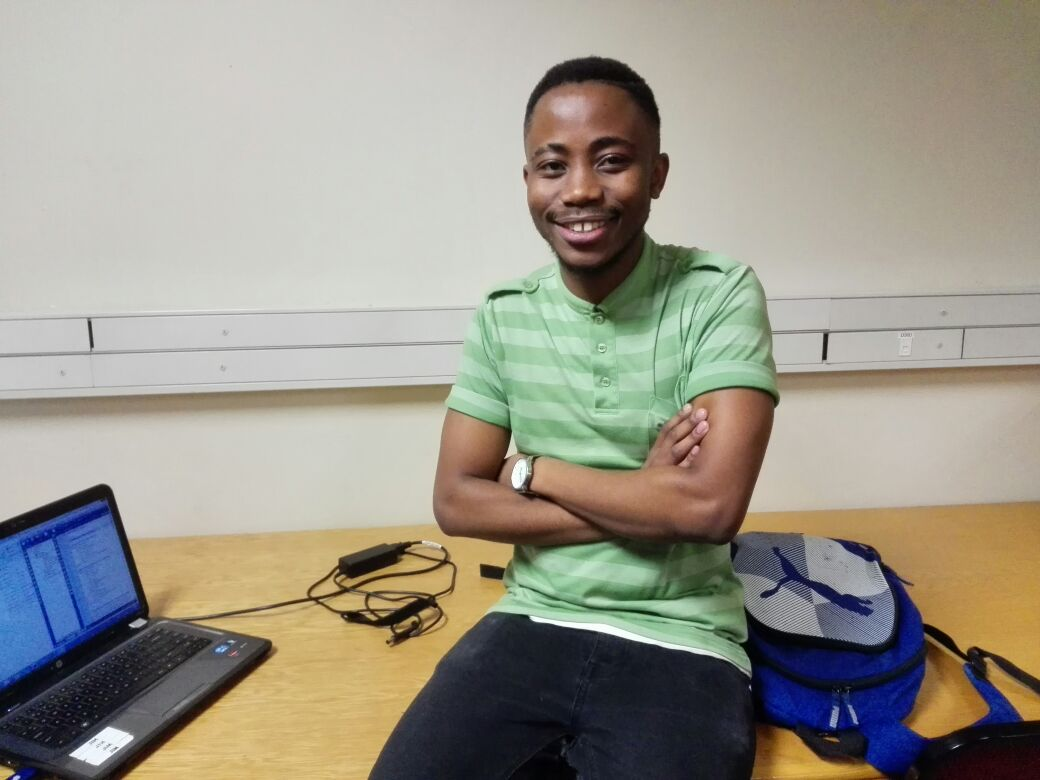
\includegraphics[width=200px]{images/Jimmy.jpg}
\end{figure}

\subsubsection{Interests:}
\begin{itemize}
	\item Chess
	\item Programming
	\item Travelling
	\item Gaming
	\item Socialising
	\item Programming Olympiads
\end{itemize}

\subsubsection{Technical Skills:}
\begin{itemize}
	\item C++
	\item Java
	\item Python
	\item C\#
	\item MySQL
	\item npm and Node.js
	\item PHP
	\item HTML, CSS
	\item XML
	\item Bootstrap
	\item Javascript
	\item Hardware Maintenance 
\end{itemize}


\subsubsection{Relevant Past Experience:}
\par{I am a two-time finalist in The Standard Bank IT Challenge. One of which my team placed third representing the University of Pretoria. This makes me confident that I can handle problems, especially in a team, whether I am under pressure or not. Synchronization and punctuality are key.}

\subsubsection{Non-Technical Strengths:}
\begin{itemize}
	\item Very approachable and charizmatic
	\item Workplace experience
	\item Diligent
	\item Problem identification and solution finding
	\item Forward and straight to the point
	\item Honest
\end{itemize}

\subsubsection{Why I chose this project:}
\par{Apart from the excitement of developing a key part of an actual instant messenger, this project broadens the horizon of the existing IM. Adding features and modifying the user interface makes me feel like part of the family that created it. The waterfall approach also aids in the ongoing research of the project.}

\newpage
%Sphe%
\subsection{Sphelele Malo}

\begin{figure}[h]
			\center
			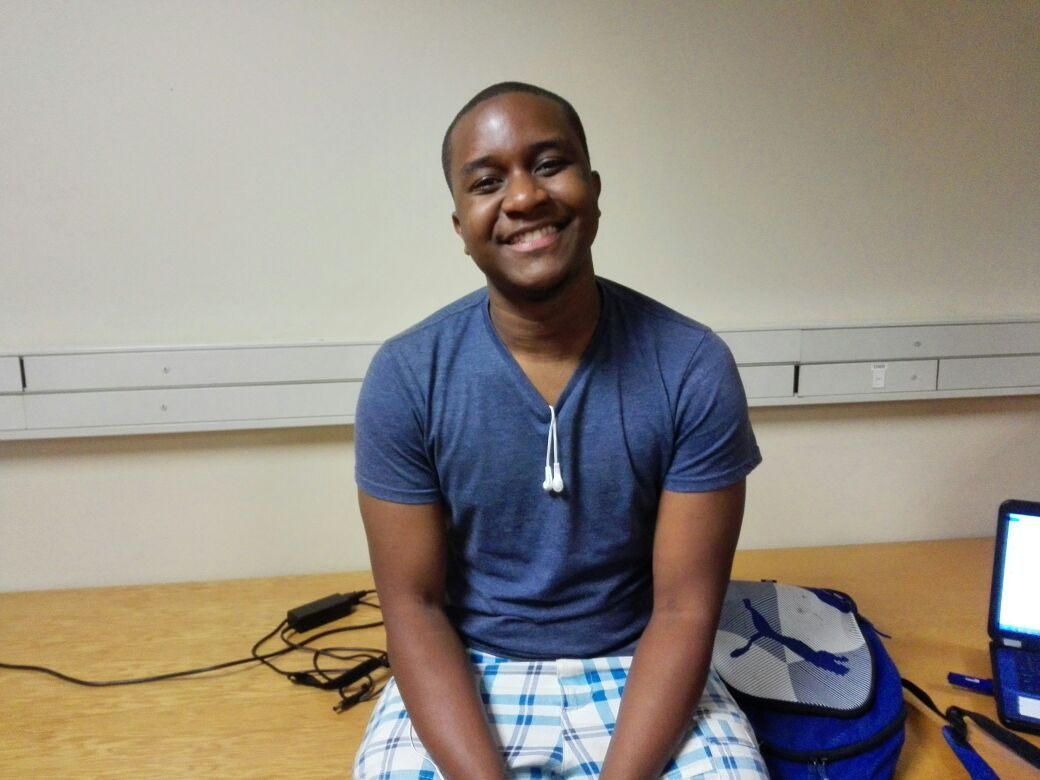
\includegraphics[width=200px]{images/sphe.jpg}
\end{figure}
\subsubsection{Interests:}
	\begin{itemize}
		\item Sports
		\item Security, networking and mobile development
		\item Gaming
		\item Listening to and the creation of music 
		\item Reading 
	\end{itemize}
\subsubsection{Technical Skills:}
	\begin{itemize}
		\item Programming (Web development, C/C++, Java)
		\item Computer and electronics 
		\item Complex problem solving
		\item Experienced with emerging technologies 
	\end{itemize}
	
\subsubsection{Relevant Past Experience:}
\par{2 week Internship at MWR Infosecurity - Web application penetration testing and lectures on mobile app security}
\subsubsection{Non-Technical Strengths:}
\begin{itemize}
		\item Teamwork
		\item Communication skills
		\item Cultural fit
		\item Responsibility and initiative
	\end{itemize}
\subsubsection{Why I chose this project:}
\par{As I listed above I have an interest in mobile app development as well as software 
security. This project would allow me to merge these two interests and both grow in experience 
and apply what I already know. I haven't been exposed to alot of mobile app development but I am a fast learner 
and am willing to fully commit to the success of this project.}

\newpage
%Armand%
\subsection{Armand Pieterse}
\begin{figure}[h]
			\center
			\includegraphics[width=200px]{images/armand.jpg}
\end{figure}
\subsubsection{Interests:}
	\begin{itemize}
		\item Computer gaming.
		\item Programming/Software development
		\item Mixed Martial Arts
		\item Electronic Technology
	\end{itemize}
		
\subsubsection{Technical Skills:}
	\begin{itemize}
		\item C++
		\item Java
		\item	C\#
		\item	MySQL
		\item	SQLServer
		\item	MongoDB
		\item PHP
		\item HTML,CSS
		\item XML
		\item Javascript and JQuery
		\item Visual Basic 
	\end{itemize}

\subsubsection{Relevant Past Experience:}
	\par{I have experience in Java and C, also I have done a mobile website/app for a 3rd year multimedia project.}

\subsubsection{Non-Technical Strengths:}
	\begin{itemize}
		\item Hard Worker.
		\item Friendly and easy to work with.
		\item Perseverance
		\item Work well in a team and alone.
		\item Self-motivated.
		\item Motivating others.
	\end{itemize}

\subsubsection{Why I chose this project:}
	\par{I have some knowledge on mobile development, but would definitely like to extend that knowledge a great deal, also I enjoy working on web- and network-based technology.I'm looking forward to be able to work on something like Linphone, I think it will be a great experience.}

\newpage
%Sito%
\subsection{Kgomotso Sito}
\begin{figure}[h]
			\center
			
\includegraphics[height=200px]{images/Kgomotso.jpg}
\end{figure}
\subsubsection{Interests:}
	\begin{itemize}
		\item Soccer
		\item Web programming
		\item Gaming
		\item Listening to music 
		\item Reading 
	\end{itemize}
\subsubsection{Technical Skills:}
	\begin{itemize}
		\item Programming
		\item Monitoring
		\item Operations and systems analysis
		\item Mathematics
		\item Computer and electronics 
		\item Complex problem solving
		\item Active listening
		\item Agile methodology
		\item Experienced with emerging technologies
	\end{itemize}
	
\subsubsection{Relevant Past Experience:}
\par{2013 – Present: vacation work with Interfront, designing customs using agile development, and did ICT support.
}
\par{Experienced C++, Java, computer security, networking, mobile development (windows) and other emerging technologies studied during my course in the university
}

\subsubsection{Non-Technical Strengths:}
\begin{itemize}
		\item Curiosity
		\item Teamwork
		\item Communication skills
		\item Cultural fit
		\item Responsibility and initiative
	\end{itemize}
\subsubsection{Why I chose this project:}
\par{I enjoy both mobile development and comfortable with java, combining the two, gives me an opportunity to make use of the skills I have learnt and at the same enjoy the experience. This makes this project ideal, not only for me but also the team. My team also shares this interest and/or view, of which is very important going forward (project development)
}

\newpage
%Ndivhuwo%
\subsection{Ndivhuwo Nthambeleni}
\begin{figure}[h]
			\center
			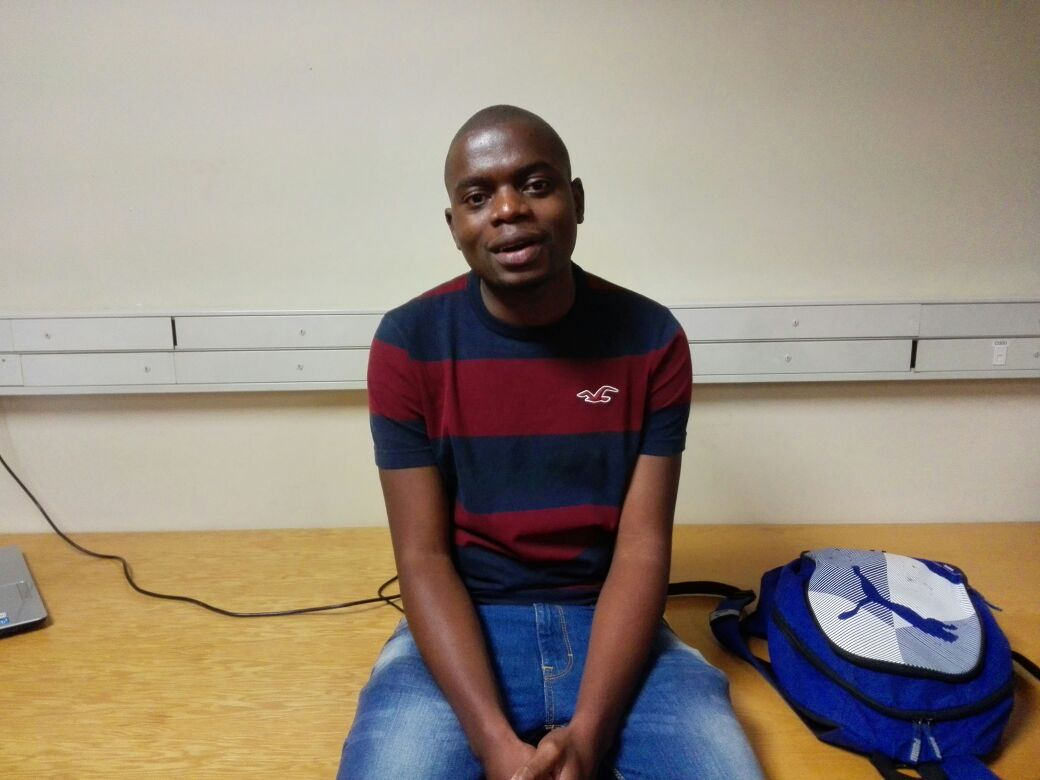
\includegraphics[width=200px]{images/Ndivhuwo.jpg}
\end{figure}
\subsubsection{Interests:}
\begin{itemize}
		\item Playing Bass guitar.
		\item Mobile development
		\item Soccer
		\item Gaming
	\end{itemize}

\subsubsection{Technical Skills:}
\begin{itemize}
		\item Programming (C++, Java, C\#, PHP (Object Oriented), HTML5, JQUERY, Python and MySQL) 1 to 4 years.
		\item Programming within the MVC, layered and Micro Kernel architectural patterns.
		\item Android Mobile Application Development 2 year
		\item Coding within the python Django and node.js frameworks.
		\item Tutoring up to 1 year
		\item Working with Linux 
		\item MS Server
		\item Advanced computer skills.
	\end{itemize}

\subsubsection{Relevant Past Experience:}
\begin{itemize}
		\item I have worked with the programming languages mentioned above for 3 years and I am quiet willing to learn new technologies that I do not have experience in.
\end{itemize}
\subsubsection{Non-Technical Strengths:}
\begin{itemize}
		\item Great Communication skills (verbal and written)
		\item Can adapt to new working environments easily.
		\item Good at identifying patterns that lead to problem solving.
\end{itemize}
\subsubsection{Why I chose this project:}
\par{I chose this project because I am looking forward to learning new technologies and enhancing my programming skills as well as applying the knowledge I have to solve problem space for this project.}
\newpage

\newpage

\section{Project Execution}
\subsection{Development Methodology}
	\par{We will be using agile methodology, because it entails the flexibility needed for such a large-scale data management system. Delivering working aspects of the system will be guaranteed to the client should the implementation be successful.}
\subsection{Client-Team Communication}
	\par{It is absolutely crucial to establish a quality communication line between the team and the client. This is so that there is synchronicity between the team's progress and the client's needs. As specified by the client, meetings will be held on a monthly basis. Any meetings in between will depend on the availability of the cient.}
\subsection{Technical Issues}
	\par{In terms of complexity, implementing a system that is easy to use and provides all the features needed by the client will be challenging. However, we will decouple front-end and back-end to hide away the complexity of the system from the user.}
	\par{The expected influx of data from multiple sources makes it challenging to process the data. It is expected in different formats and a generic accepting feature has to be implemented. Enforcing the ISDA FPML standard will help a great deal in achieving a solution for the aforementioned problem.}
\subsection{Technologies}
	\par{C\# will be the language of choice using Visual Studio IDE. As well as all the technologies specified by the client (e.g. Hadoop and mulesoft). As development planning commences, other optimal technologies will be defined to accommodate the needs of the system.}
\subsection{Deliverables}
	\begin{itemize}
		\item A working system
		\item A working service with each client-team meeting
		\item Source code
		\item Documentation
	\end{itemize}
\end{document}